\documentclass[a4paper,12pt]{article}
\usepackage[utf8]{inputenc}
\usepackage[brazil]{babel}
\usepackage{hyperref}
\usepackage{graphicx}
\usepackage{amsmath}
\usepackage[hmarginratio=1:1,top=40mm,columnsep=20pt]{geometry}

\title{Universidade Federal do Paraná \\
    Bacharelado em Ciência da Computação \\
    Tópicos em Reconhecimento de Padrões \\
    \textbf{Combinação de Classificadores de Assinaturas}}

    
\author{\href{mailto:fhbz10@inf.ufpr.br}{Flávio Henrique de Bittencourt Zavan}\\ e \\
    \href{mailto:trcl10@inf.ufpr.br}{Thiago Roscia Cerdeiro de Lima} \\
    Professor: Luiz Eduardo S. Oliveira}

\begin{document}
\maketitle

\section*{Introdução}
Para o trabalho da matéria Tópicos em Reconhecimento de Padrões, a proposta se
resumiu em classificar novas assinaturas de acordo com uma base de treino,
fazendo uso de dois classificadores. 

\section*{Objetivos}
\begin{itemize}
    \item Dividir e normalizar base
    \item Extrair Características
    \item Implementar os classificadores
    \item Combinar as saídas
    \item Gerar Matriz de Confusão e Curva \textit{ROC}
\end{itemize}

\section{Desenvolvimento}
Como várias peças de quebra-cabeça, o trabalho não requeriu uma ordem certa
para ser montado. Portanto, aproveitando o fato de o \textit{K-NN} (\textit{-Nearest Neighbors}
 já ter sido implementado, o trabalho foi iniciado por sua adaptação e
logo começou-se a seleção de características.\\
Após alguns testes utilizando a Matriz de Confusão para analisar
o desempenho do \textit{K-NN}, definiu-se uma padronização para a utilização da base e das
 entradas e saídas. Foi implementado, então, o \textit{Perceptron} e, por fim, gerada a
 curva \textit{ROC} (\textit{Receiver Operating Characteristic}).

\section{Divisão e Normalização da Base}
Inicialmente, os testes do \textit{K-NN} foram feitos treinando toda a base que
se tinha em mão e testando cada um dos casos com todos os outros. Ou seja,
eram feitos 261 testes, cada um com uma base de tamanho 260.\\
Foi criado, então, um script em \textit{shell} para gerar 9 sub-bases (pois, para cada
autor, temos 9 exemplos), onde, em cada uma delas, um exemplo de cada autor 
não seria utilizado para treinamento, apenas para teste. Com 9 bases de treino
e, para cada uma delas, 9 casos de teste, totalizou-se 81 casos de teste únicos
para a avaliação do desempenho do trabalho.\\
Foi utilizada a normalização \textit{Min-Max} e, não apenas a base normalizada é 
salva, quanto os parâmetros "min" e "max" de cada característica também são para
 normalizar, posteriormente, os casos de teste.

\section{Extração de Características}
Escolher e testar as características que melhor descrevessem a singularidade das
 assinaturas foi, provavelmente, a etapa que mais tomou tempo. Começou-se
pelo básico: segmentar as imagens e aplicar pequenos filtros para retirar
alguns ruídos. Analisando a base, logo notou-se diferenças significativas na
relação \textit{altura / largura} e escolheu-se essa razão como uma
característica. Quantidade de componentes pretas conexas (quantas 
"\textit{palavras}" há na assinatura) e quantidade de regiões brancas totalmente
 envoltas por pretas (como a volta do '\textit{g}' e do '\textit{l}' cursivos)
foram outras duas características que chamaram a atenção.\\
Calculou-se, também, a direção dos pixels, mas apenas considerando se havia pixel
 à esquerda ou à direita pois, em muitos casos, havia uma grande região branca
 em cima e em baixo, o que geraria vários casos com características iguais. Para
 essa característica, dividiu-se as imagens em regiões, mas ainda tomando cuidado
 com a quantidade para evitar um vetor muito grande, já que este poderia
 resultar na maldição da dimensionalidade.\\
Testando os resultados com o \textit{K-NN}, optou-se por trocar essas últimas
características pela posição do pixel preto mais alto e pela do pixel preto mais
 baixo em cada região. Apesar de parecer mais simples, essa característica
 demonstrou-se uma melhor descritora das imagens. Testando para quantidade de
 regiões diversas, obteve-se melhor resultado com uma divisão de 16 regiões.\\
Ficou-se, então, com duas coordenadas por região mais as três características
 supracitadas, resultando em um vetor de tamanho 35.

\section{Implementação dos Classificadores}
\subsection{\textit{K-NN}}
O algoritmo do \textit{K-NN} segue o modelo visto em sala e previamente implementado.
Ele recebe como parâmetros o nome do arquivo da base normalizada, o \textit{K}
e o caso de teste. Através da base, ele conta a quantidade de elementos e de
características, assim como lê os parâmetros para normalização do caso de teste.
 Após a leitura e normalização deste, o programa calcula a distância euclidiana
para todos os casos da base de treinamento e imprime o K mais próximos. 

\subsection{\textit{Perceptron}}
A princípio, cogitou-se implementar o \textit{Perceptron} para classificar dentre todas 
as 29 classes. Entretanto, dado o bom resultado que se obteve apenas com o \textit{K-NN},
 optou-se por utilizar o \textit{Perceptron} binário com o intuito de resolver os casos em 
que o \textit{K-NN} achou 50\% de chances entre duas classes (quando \textit{K = 2}). O
 \textit{Perceptron} recebe como parâmetros a base de treino normalizada, as 2 classes 
impressas pelo \textit{K-NN} e o caso de teste. Se as classes forem iguais, ele ignora, 
pois o KNN já tomou a decisão. Caso sejam diferentes, o \textit{Perceptron} faz
 \begin{math}n^2\end{math}
 iterações de aprendizado para atualizar os pesos e o \textit{bias} para então
aplicá-los nas características do caso de teste e tomar a decisão utilizando o 
\textit{hardlim()}. 

\subsection{Combinação de saídas}
Como dito previamente, a entrada do \textit{Perceptron} depende da saída do \textit{K-NN}. Ou 
seja, optou-se pela combinação sequencial. Foi criado um script em \textit{shell} que
 automatiza a execução dos programas e filtra a saída do \textit{K-NN} para alimentar o
 \textit{Perceptron}.

\section{Matriz de Confusão e Curva \textit{ROC}}
Para avaliar o desempenho dos classificadors, fez-se uso de uma Matriz de
 Confusão e imprimiu-se a porcentagem de acertos. Com isso, foi possível avaliar
 casos específicos onde havia confusão entre classes para encontrar
 características que as distinguissem.\\
A Curva \textit{ROC} só foi gerada ao final da implementação de todo o resto.

\section{Resultados Obtidos}
O classificador inicial, fazendo uso das características mais simples, 
começou com uma taxa de 86\% de acerto. Com a utilização da direção dos pixels, 
a taxa chegava a 94\%, com \textit{K=3} e 4 regiões. Trocando a direção dos pixels pela 
posição dos pixels mais alto e mais baixo, conseguiu-se alcançar 100\% de 
reconhecimento apenas com o \textit{K-NN} (para 16 regiões e \textit{K=1}). Com \textit{K=2}, a taxa 
continuava, teoricamente, em 100\%. Porém, em casos em que havia dúvida, ele 
considerava como \textit{K=1}. Para resolver isso, utilizou-se o \textit{Perceptron}, que manteve 
a taxa de acerto em 100\%.\\
Isso resultou na plotagem da curva mostrada na Figura 1.

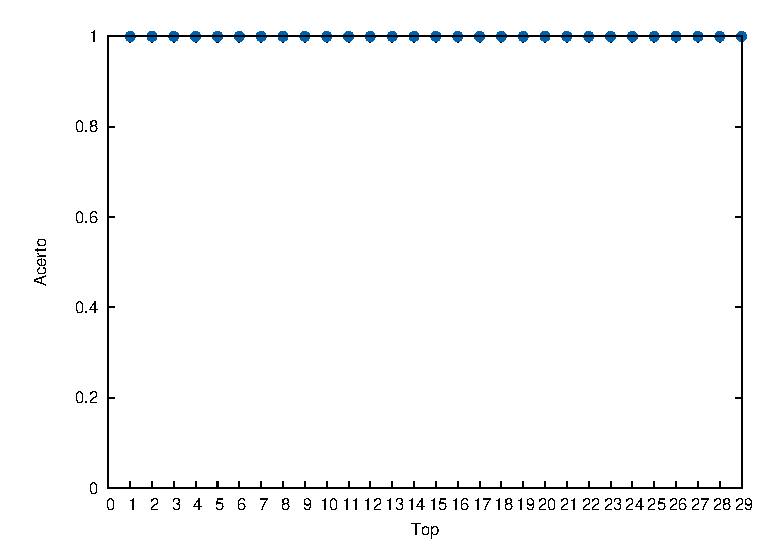
\includegraphics{roc.eps}

\end{document}
